\documentclass{beamer}
\usepackage[utf8]{inputenc}
% \usepackage{default}
% \usepackage{paralist}
% \usepackage{enumitem}
\usepackage{changepage}
\usepackage{color, colortbl}
\usepackage{enumerate}
% \setlist{align=left}
\usetheme{Warsaw}
\usecolortheme{beaver}
% \usetheme{Antibes}
\geometry{paper=a4}
\def\Put(#1,#2)#3{\leavevmode\makebox(0,0){\put(#1,#2){#3}}}
\setbeamertemplate{navigation symbols}{}   
\setbeamertemplate{footline}{}   

\definecolor{Gray}{gray}{0.9}
\definecolor{GrayOscuro}{gray}{0.71}
\definecolor{celestito}{rgb}{0.88,1,1}

\title{PATENA: an algorithm for the design of protein linker sequences}
\date{}

\author{Ignacio Eguinoa, Ignacio Enrique Sánchez}
\institute[VFU] % (optional)
{ Protein Physiology Laboratory, Departamento de Química Biológica, Facultad de Ciencias Exactas y Naturales and IQUIBICEN-CONICET, Universidad de Buenos Aires, Buenos Aires, Argentina}

\begin{document}











% *********************************************
%            START 
% *********************************************
\begin{frame}
 \titlepage
% \includegraphics[width=70px]{../img/logofcen.pdf} 
\hspace{4px}
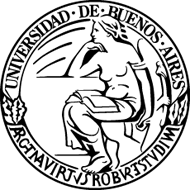
\includegraphics[width=55px,height=50px]{../img/logouba.png}
\hspace{50.7px}
% \centering

\includegraphics[width=70px,height=50px]{../img/logoCONICET.jpg} 
\hspace{15px}

\includegraphics[width=100px,height=50px]{../img/logoLFP.jpeg}
\end{frame}










\begin{frame}[plain]{Chimeric proteins}
%  Many proteins in nature are multidomain \\
%  use of protein engineering process to covalently join 2+ proteins/domains
%  New construction made of 2+ proteins/domains\\
 %  \Put(0,10)
%  \vspace{-3.5\baselineskip}


% for example, we have here 2 fluorescent domains(Cyan fluorescent protein and yellow fluorescent protein)
% When 2 fluorescent proteins/domains) are sufficiently separated, they retain their spectral properties.

% FRET dependence with distance\\
Cyan Fluorescent Protein(CFP) - Yellow Fluorescent Protein(YFP)\\
 \begin{adjustwidth}{-1.5em}{-3.5em}
 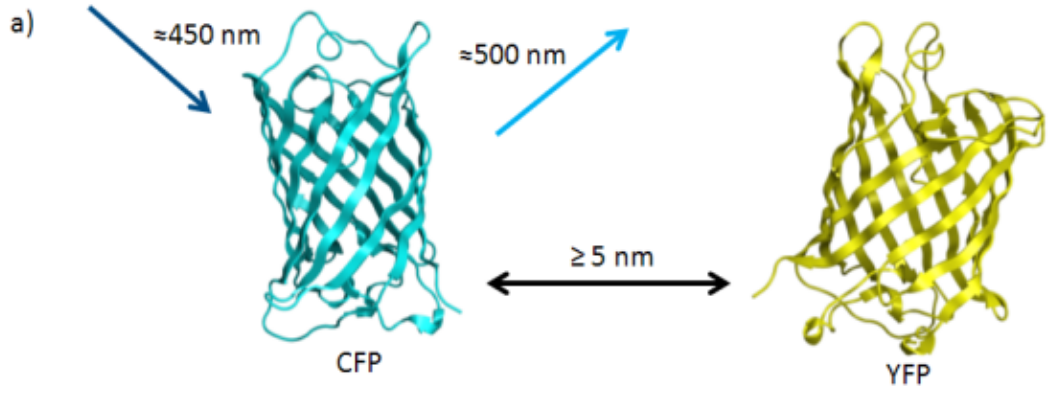
\includegraphics[width=170px]{../img/fretDomainsA.png}
 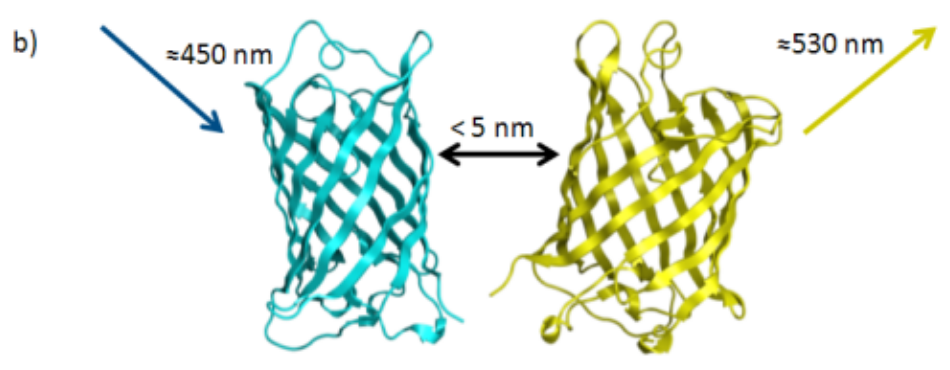
\includegraphics[width=170px]{../img/fretDomainsB.png}
\end{adjustwidth}
Distance-dependent spectral properties\\
  \vspace{10px}
Macromolecular crowding sensor:  CFP + Linker + YFP \\
\vspace{10px}
% Multiple molecular sensors:  YFP -  
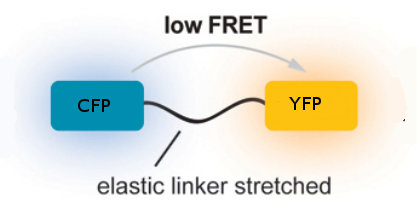
\includegraphics[width=125px,height=60px]{../img/fretSeparadosCFP.png}
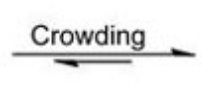
\includegraphics[width=80px]{../img/crowdingSign.png}
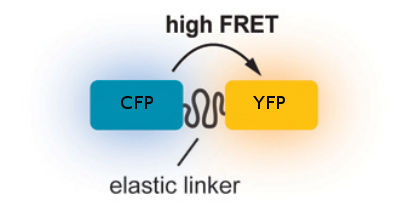
\includegraphics[width=125px]{../img/fretJuntosCFP.png}
% one construction(one macrmolecule) function as a sensor
%   \centering
%  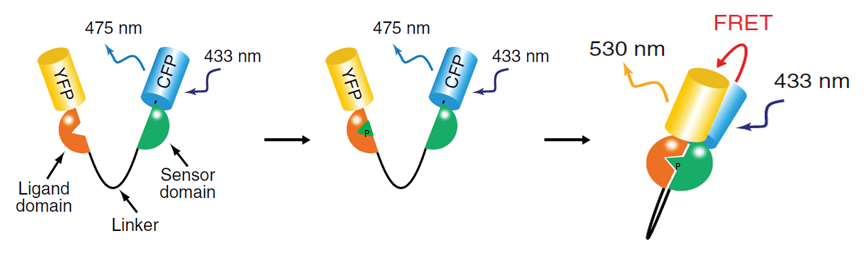
\includegraphics[width=330px]{../img/fret.png}
\end{frame}

% These construcions are 

% QUE SON
% ejemplos:
% 	Formación de proteinas bifuncionales mediante union covalente de dominios.
% 	Promover la unión entre proteinas que forman complejos, generando una unión covalente entre ellos
% 
% proceso de sintesis:
% 	-unir los dominios de interes
%       -clone into expression system










\begin{frame}{Relevant linker properties}
% From this example application(fret sensors) we see that, besides defining the domains to be linked, we need to define a linker sequence.
%  a linker is a sequence with a very important function....it allows the domains to remain covalently linker while folding in an independent manner, moving and interacting freely
\vspace{-20px}
\begin{adjustwidth}{-0.5em}{-1.5em}
\textbf{Allows domains to fold independently, move and interact freely}
 \end{adjustwidth}

 \vspace{10px}

\begin{itemize}
  \item Length
  \item Remain in a flexible conformation  %incluye prevencion de aggregation
    \begin{itemize}
     \item Disordered structure, Non-aggregating
    \end{itemize}

  \item Biologically inert  %lack of functional features
  \item Other desirable aspects  %experimental aspects
    \begin{itemize}
     \item AAs frequencies, UV silent, net charge
%   Composition
    \end{itemize}
\end{itemize}

% \Large{....linker design is not a trivial problem}

\end{frame}











\begin{frame}{Current approaches to linker design}
\begin{itemize}

\item Use linkers from natural multi-domain proteins


\item Intuitive design.
%  there are lots of chimeric constructions that were experimentally tested....reuse. may involve small engineering process to adapt the sequence(lenght, composition, etc)
 \begin{itemize}
%   \item Reuse from literature or propose novel sequence. 
  \item Usually (G/S/P)-rich 
%   \begin{itemize}
%    \item  i.e $(GGGS)_n$ 
  \end{itemize}
%     \end{itemize}

\item Pseudo-Rational design. 
\begin{itemize}
 \item Servers: LINKER, Linkerdb, SynLinker.
\end{itemize}

%      DB (natural/previously used designs)
%     these include from different collections obtained in different projects	

%   \item Very limited set of sequences and composition
%  \subitem Requires experimental test (prueba y error) 
% \begin{itemize}
%  \item 
\end{itemize}
\vspace{20px}
\LARGE{Structure? Inert? Diversity?}
% \end{itemize}
\end{frame}















% \section{Method}

\begin{frame}{Rational approach}
% No method can provide a clean design\\ % a design clean of unwanted properties
 
% If we have a candidate linker sequence...
PATENA uses different applications to evaluate a candidate linker.
\vspace{15px}
% all apsects associated with linker properties can be assses by means of different bioinformatic tools available, that can analyze the sequence
% a pesar que los requerimientos no son muuchos, es decir, podemos asumir que gran cantidad de secuencias podrian funcionar como linkers

% We can evaluate (get an idea, get an estimation of) how good or how bad(quality) is a sequence to work as a linker.
% We can predict all unwanted properties.
\begin{tabular}{l|l}
\textbf{Undesired feature} & \textbf{Prediction method} \\ \hline \hline
\rowcolor{Gray} Globular structure & IUPred  \\
Aggregate structure & TANGO, PASTA, WALTZ   \\
\rowcolor{Gray}Functional features & BLAST, ELM, PROSITE, ANCHOR \\  
UV absorbers(OPTIONAL) & Presence of UV-absorbers residues \\
\rowcolor{Gray}Net charge(OPTIONAL)& Presence of charged residues\\
\end{tabular}
 
% \Large{Use this information to aid in linker design process}
\vspace{20px} 
% DECIR QUE TODOS LOS MÉTODOS DAN INFORMACION A NIVEL DE POSICION DENTRO DE LA SECUENCIA
%  any of these methods allows to define if a particular position contains a specific negative aspect 
% each of these methods allows to asses if a particular position has that specific negative aspect we are evaluating
% so we can define a scoring function
Each of these methods allows to predict the presence of undesired features at specific position $\rightarrow$ define a scoring function
% Each method predicts the presence of undesired features at position level $\rightarrow$ we can define a scoring function
% \vspace{10px}
 
% once we have a scoring function, we add a method to 

% Use heuristic approach(Monte Carlo): \\
% \textbf{Input}
% (User's sequence / Random sequence) $\rightarrow$ (Sequence with score=0)




\end{frame}






% ESTO ES BASICAMENTE EL FUNDAMENTO DEL MÉTODO
% if we want to use this aspects to evaluate
% para usar esta informacion necesitamos 2 cosas
% 1 - formalize this estimation idea...i mean, we can get automatize and quantify the evaluation 
% AND
% 2 - find a good way to search for candidate sequences , to evaluate if they have the desired properties.
%	 we (probably) cant just start testing random sequences and see if they work...it would be highly inefficient
%	 we cant use natural sequences because, as we said, they dont always fulfill our needs
% 
% if we can find these 2 things we will have a design method
% 
% what is more, in our application these 2 aspects are connected !!!



% ACA EXPLICO EL PUNTO 1 - CUANTIFICACION DE LA CALIDAD 
% \begin{frame}{Linker evaluation}
% \begin{itemize}
% 
% %  Turn the evaluation schema into a function $f(sequence) -> score$
% % quantify using discrete values
%  \item Turn the estimation into a scoring function by calculating the undesired features\\
% % Penalize unwanted properties\\
% % Quantify how good(or bad) is a sequence
% 
% % quantify de quality of the sequence
% % es decir...if we define a function f(face)
% %   
% %   \item Higher score $\rightarrow$ unwanted properties $\rightarrow$ worse linker
%   
%  \item Score $\geqslant 0$ (Higher score $\rightarrow$ bad linker)
% % we dont really care how high or low is the score, we want a linker with score = 0
% \end{itemize}
% 
% % ES IMPORTANTE DESTACAR QUE EL PROCESO DE EVALUACIÓN CAN BE ADAPTED TO ANY RELEVANT ASPECT THAT WANT TO BE ASSESED
% % IF YOU THINK THAT ITS GONNA BE RELEVANT THAT ASSES 
% % \vspace{0.3cm}
% % \begin{adjustwidth}{-1.5em}{-2.5em}
%  
% 
% % \end{adjustwidth}
% \end{frame}





% 
% % dijimos que queriamos usar esta informacion (el score) to aid in linker design
% \begin{frame}{Linker design}
% % the second thing we need is 
% % ahora que definimos un score
% \begin{itemize}
%  \item Aiming at sequence with Global score = 0.
%   
%  \item We have information for each position and the whole sequence
% %  \item We have information of quality(score) at sequence level (detalied for each position).
%  
% \end{itemize}
% 
% %  TENEMOS INFORMACION SOBRE DETALLADA A NIVEL DE RESIDUO(NO SOLO EL SCORE GLOBAL)
% % we can use this information to guide the search
% 
% % so, we propose a search method 
% % We propose a search method: 
% % to search for (optimal) sequence 
% \begin{enumerate}
%  \item Propose tentative linker as starting sequence 
% %     \begin{itemize}
% %     \item Random sequence works too! (\textit{de novo} design)
% %     \end{itemize}
%    
%  \item Propose point mutations to high scoring positions
% %  we will get back to this later
%       \begin{itemize}
%       \item If score decreases $\rightarrow$ incorporate mutation to design.  
%       \item If NOT $\rightarrow$ heuristic decision (Score difference $\rightarrow$  $A_{rate}$).  
%      \end{itemize}
%       
%  \item Repeat step 2 until score=0
% \end{enumerate}
% 
% 
% % $\beta=k_b Temp$  POR LO TANTO, A MAYOR Temp, MAYOR BETA Y POR LO TANTO MAYOR FRECUENCIA DE ACEPTACION
%  
% \Large{Random sequences can work too! (\textit{de novo} design)}\\
% \vspace{7px}
%  
% \Large{Obtaining a design is now an optimization problem}
% 
% 
% % and we are trying to apply an heuristic search method
% 
% % SOLVING AN OPTIMIZATION PROBLEM MIGHT HAVE DIFFERENT SOLUTIONS
% % una aproximacion mediante mutaciones permitiria buscar soluciones similares a una secuencia inicial definida por el usuario
% % ademas, mediante el control de la frecuencia de aminoacidos podriamos controlar la composicion
% 
% \end{frame}


% *********************************************
%      EJEMPLO DE EVALUACION DE SCORE
% *********************************************

% ACA DIGO: YA QUE TENEMOS LAS HERRAMIENTAS DISPONIBLES PARA LA EVALUACION Y UN METODO GENERAL PARA ENCONTRAR UNA SECUENCIA FINAL, DETALLAMOS CUAL ES LA FUNCION DE SCORING
% 
\begin{frame}{Scoring example}
 \begin{tabular}{llllllllllllll} 
\hline
\rowcolor{GrayOscuro}Sequence & \textbf{M} & \textbf{V} & \textbf{L} & \textbf{S} & \textbf{P} & \textbf{A} & \textbf{D} & \textbf{K} & \textbf{T} & \textbf{N} & \textbf{P} & \textbf{D} \\ \hline \hline
 
% Puntaje Inicial & 0 & 0 & 0 & 0 & 0 & 0 & 0 & 0 & 0 & 0 & 0 & 0\\ \hline
\rowcolor{Gray}IUPred           	& 0 & 1 & 1 & 1 & 1 & 0 & 0 & 1 & 1 & 1 & 0 & 0\\ \hline  
TANGO 		       			& 1 & 1 & 1 & 1 & 0 & 0 & 0 & 0 & 0 & 0 & 0 & 0\\ \hline  
\rowcolor{Gray}PASTA			& 1 & 1 & 0 & 0 & 0 & 0 & 0 & 1 & 0 & 1 & 1 & 1\\ \hline  
ELM          	      			& 0 & 1 & 1 & 0 & 0 & 0 & 0 & 1 & 1 & 1 & 1 & 1\\ \hline 
\rowcolor{Gray}BLAST			& 1 & 0 & 1 & 1 & 1 & 0 & 0 & 0 & 0 & 1 & 1 & 1\\ \hline 
PROSITE 	      			& 0 & 0 & 1 & 0 & 0 & 0 & 0 & 0 & 0 & 1 & 1 & 1\\ \hline 
\rowcolor{Gray}ANCHOR	        	& 1 & 1 & 1 & 0 & 0 & 0 & 0 & 0 & 0 & 1 & 0 & 1\\ \hline \hline
\rowcolor{GrayOscuro}Position score     & 4 & 5 & 6 & 3 & 2 & 0 & 4 & 3 & 2 & 6 & 4 & 5\\ \hline
\rowcolor{GrayOscuro}Global Score  & 44 &&&&&&&&&&& \\ \hline
\end{tabular}
\end{frame}






% *********************************************
%      ESQUEMA GRAFICO DE PATENA
% *********************************************
\begin{frame}[plain]{PATENA method}
% \vspace{-0.5\baselineskip}
\begin{adjustwidth}{-2.0em}{-2.0em}
% \begin{adjustheight}{-1.5em}{-1.5em}
% 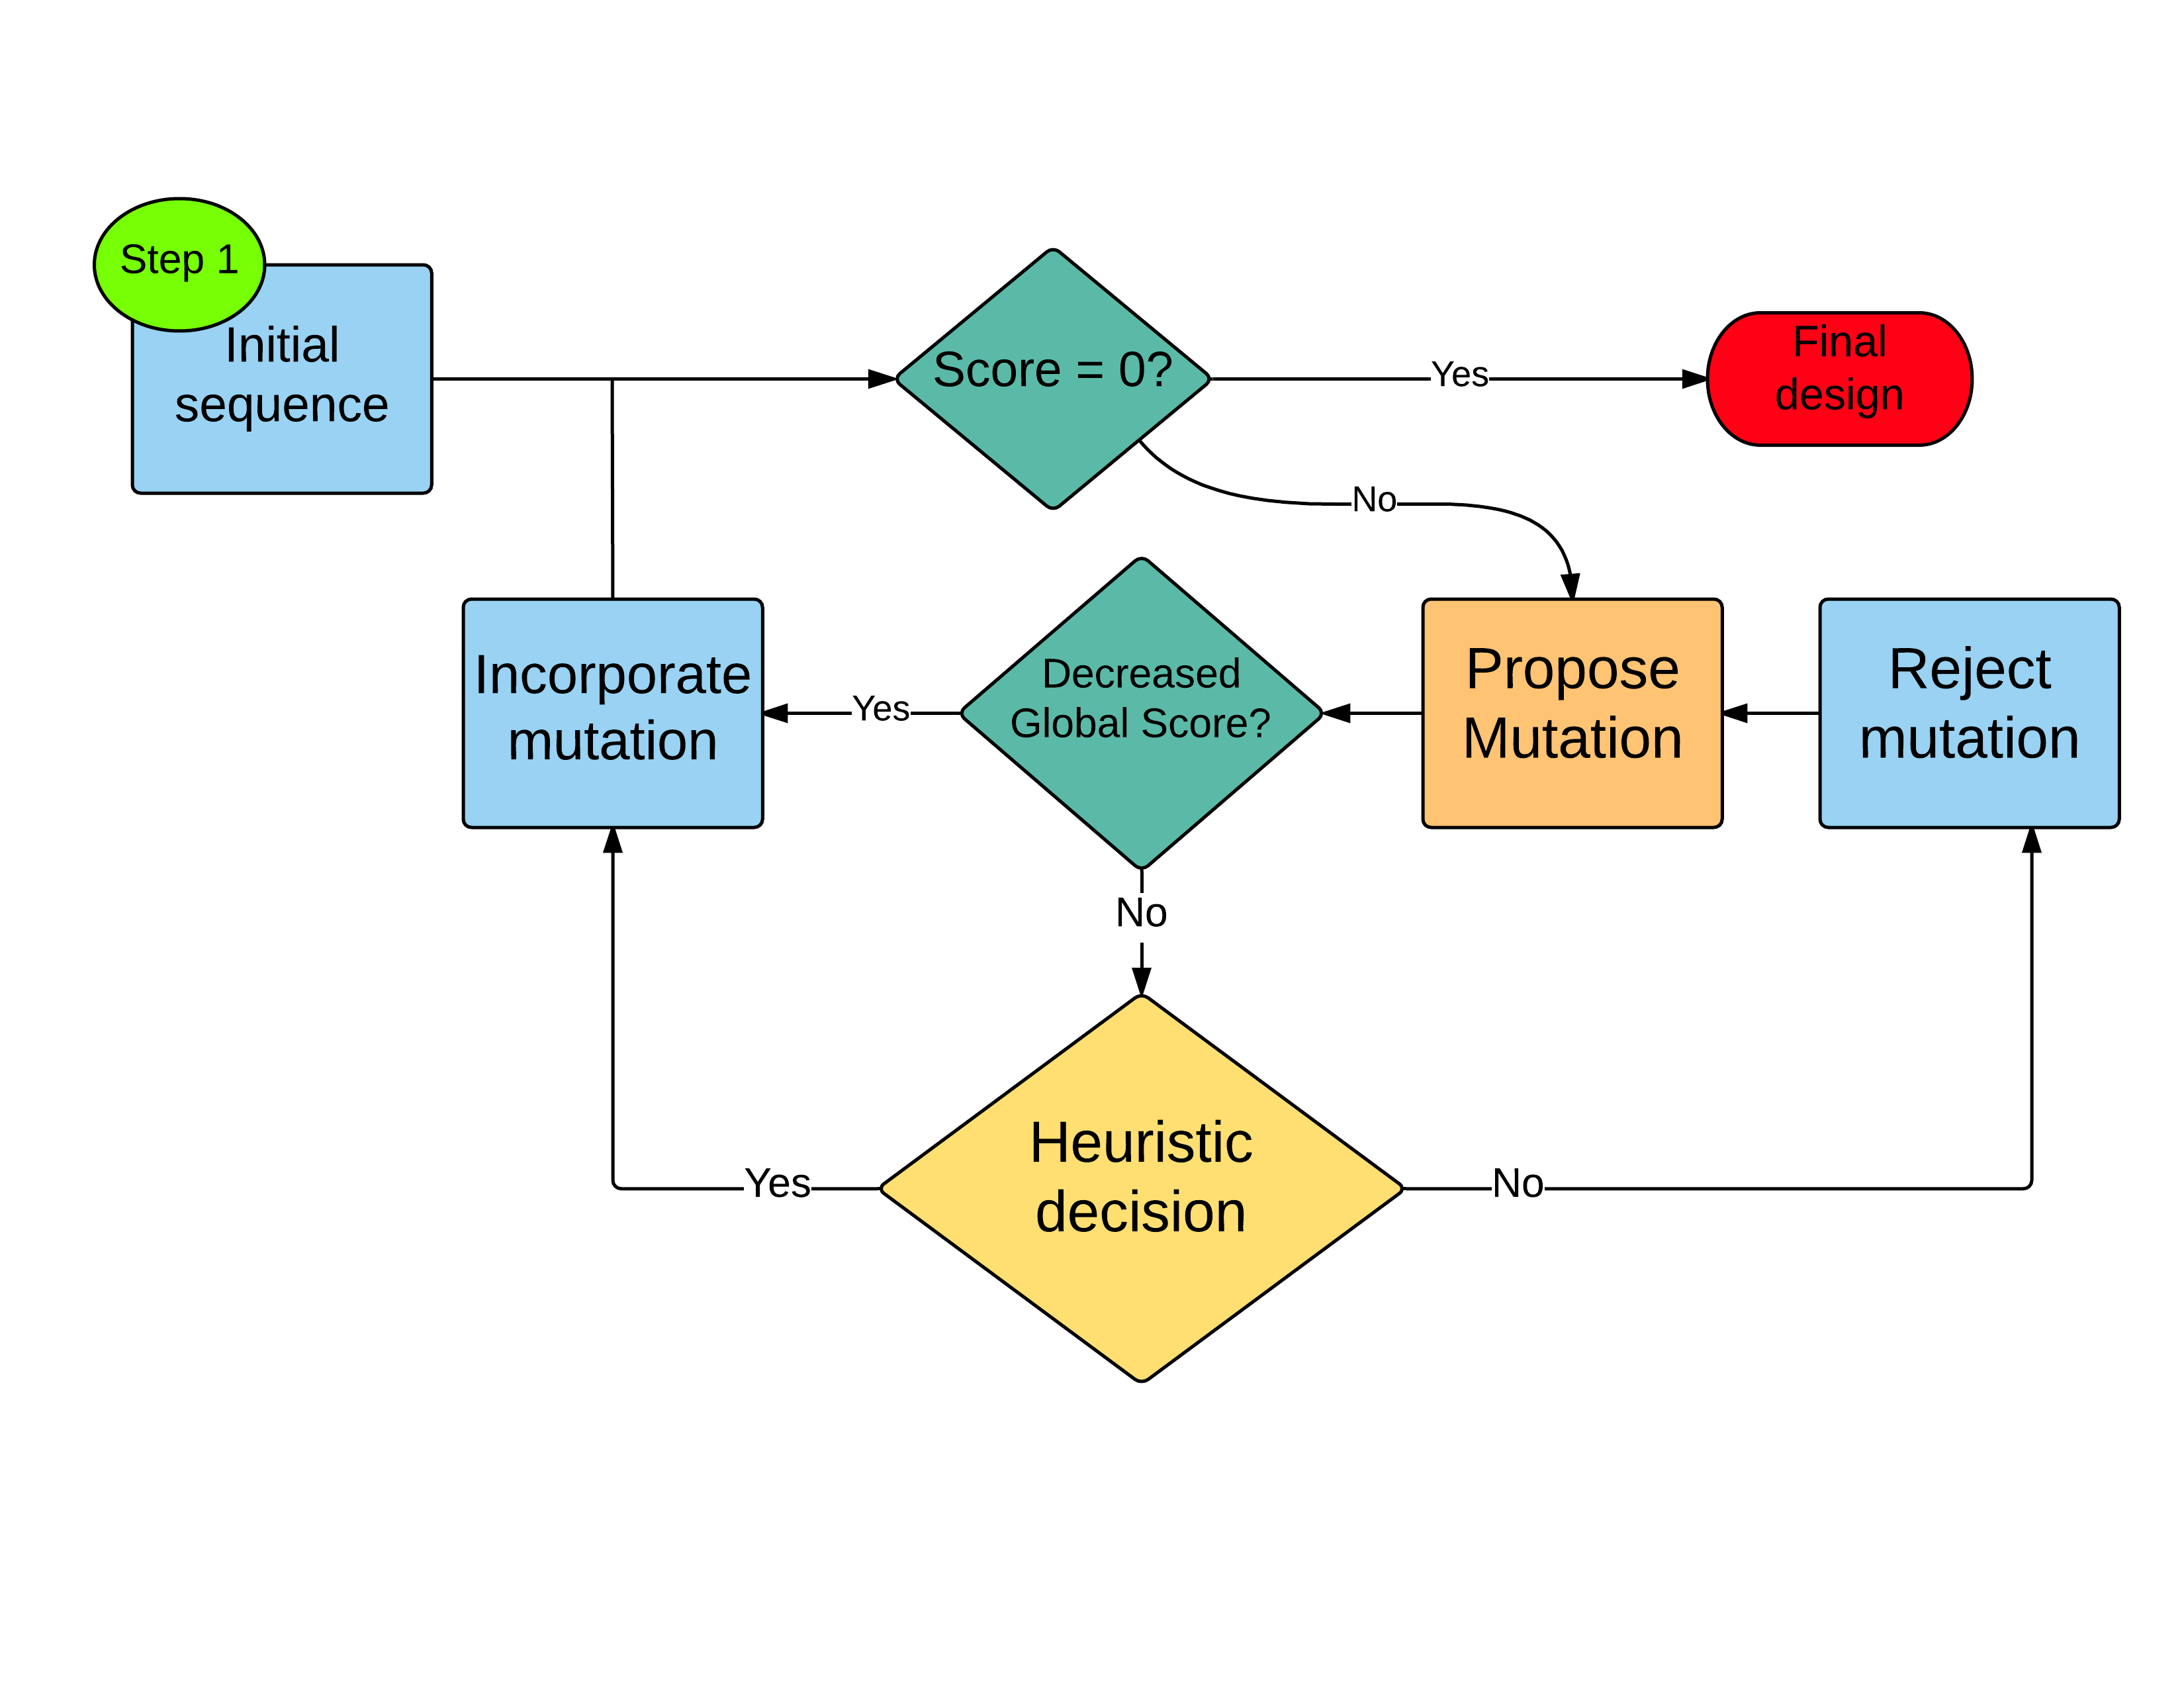
\includegraphics[width=350px,height=250px]{../img/patenaReduced.png} 
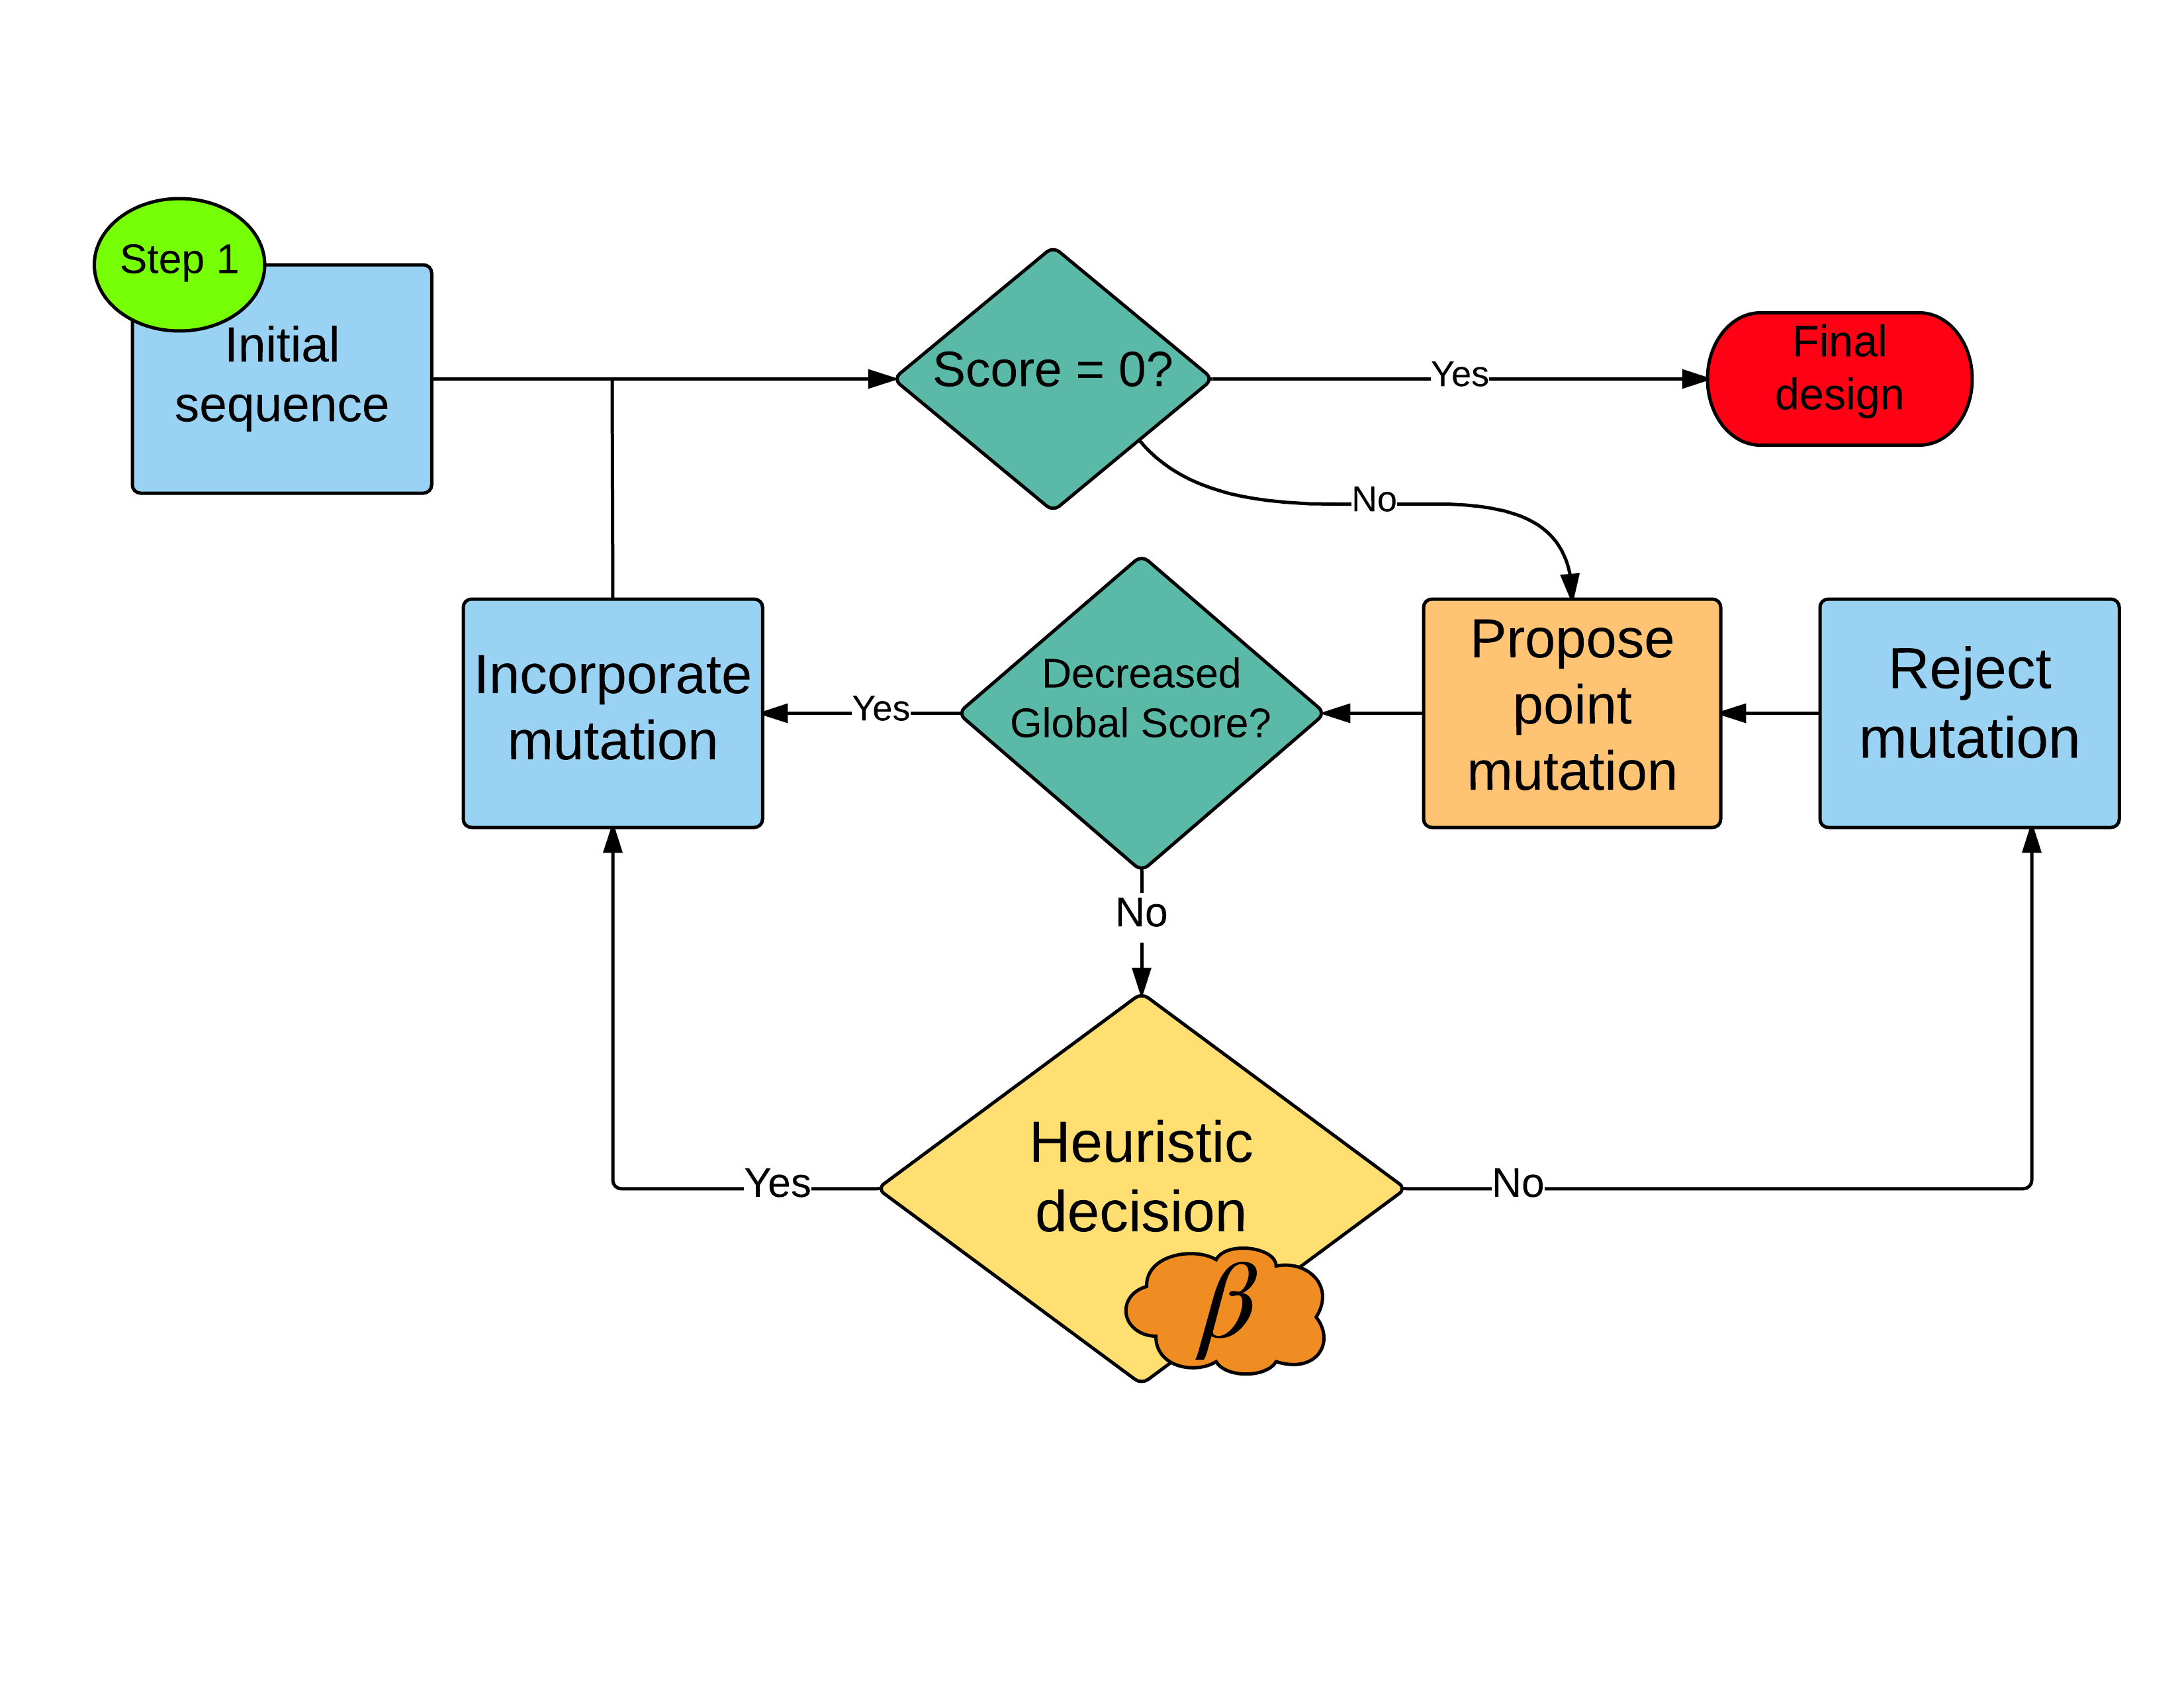
\includegraphics[width=350px,height=250px]{../img/patenaReduced-Beta.png} 
% \end{adjustheight}
\end{adjustwidth}
% \vspace{-\baselineskip}
\end{frame}

























% *********************************************
%      BETA vs TIME
% *********************************************
\begin{frame}[plain]{Effective $\beta$ range $\approx$ [0.1 - 2.0]}
\centering
% Optimal $\beta$ range  
[Length = 50] - [Random (n=3) and Natural (n=3) seq. / each $\beta$] \\
\begin{adjustwidth}{-1.5em}{-2.5em}
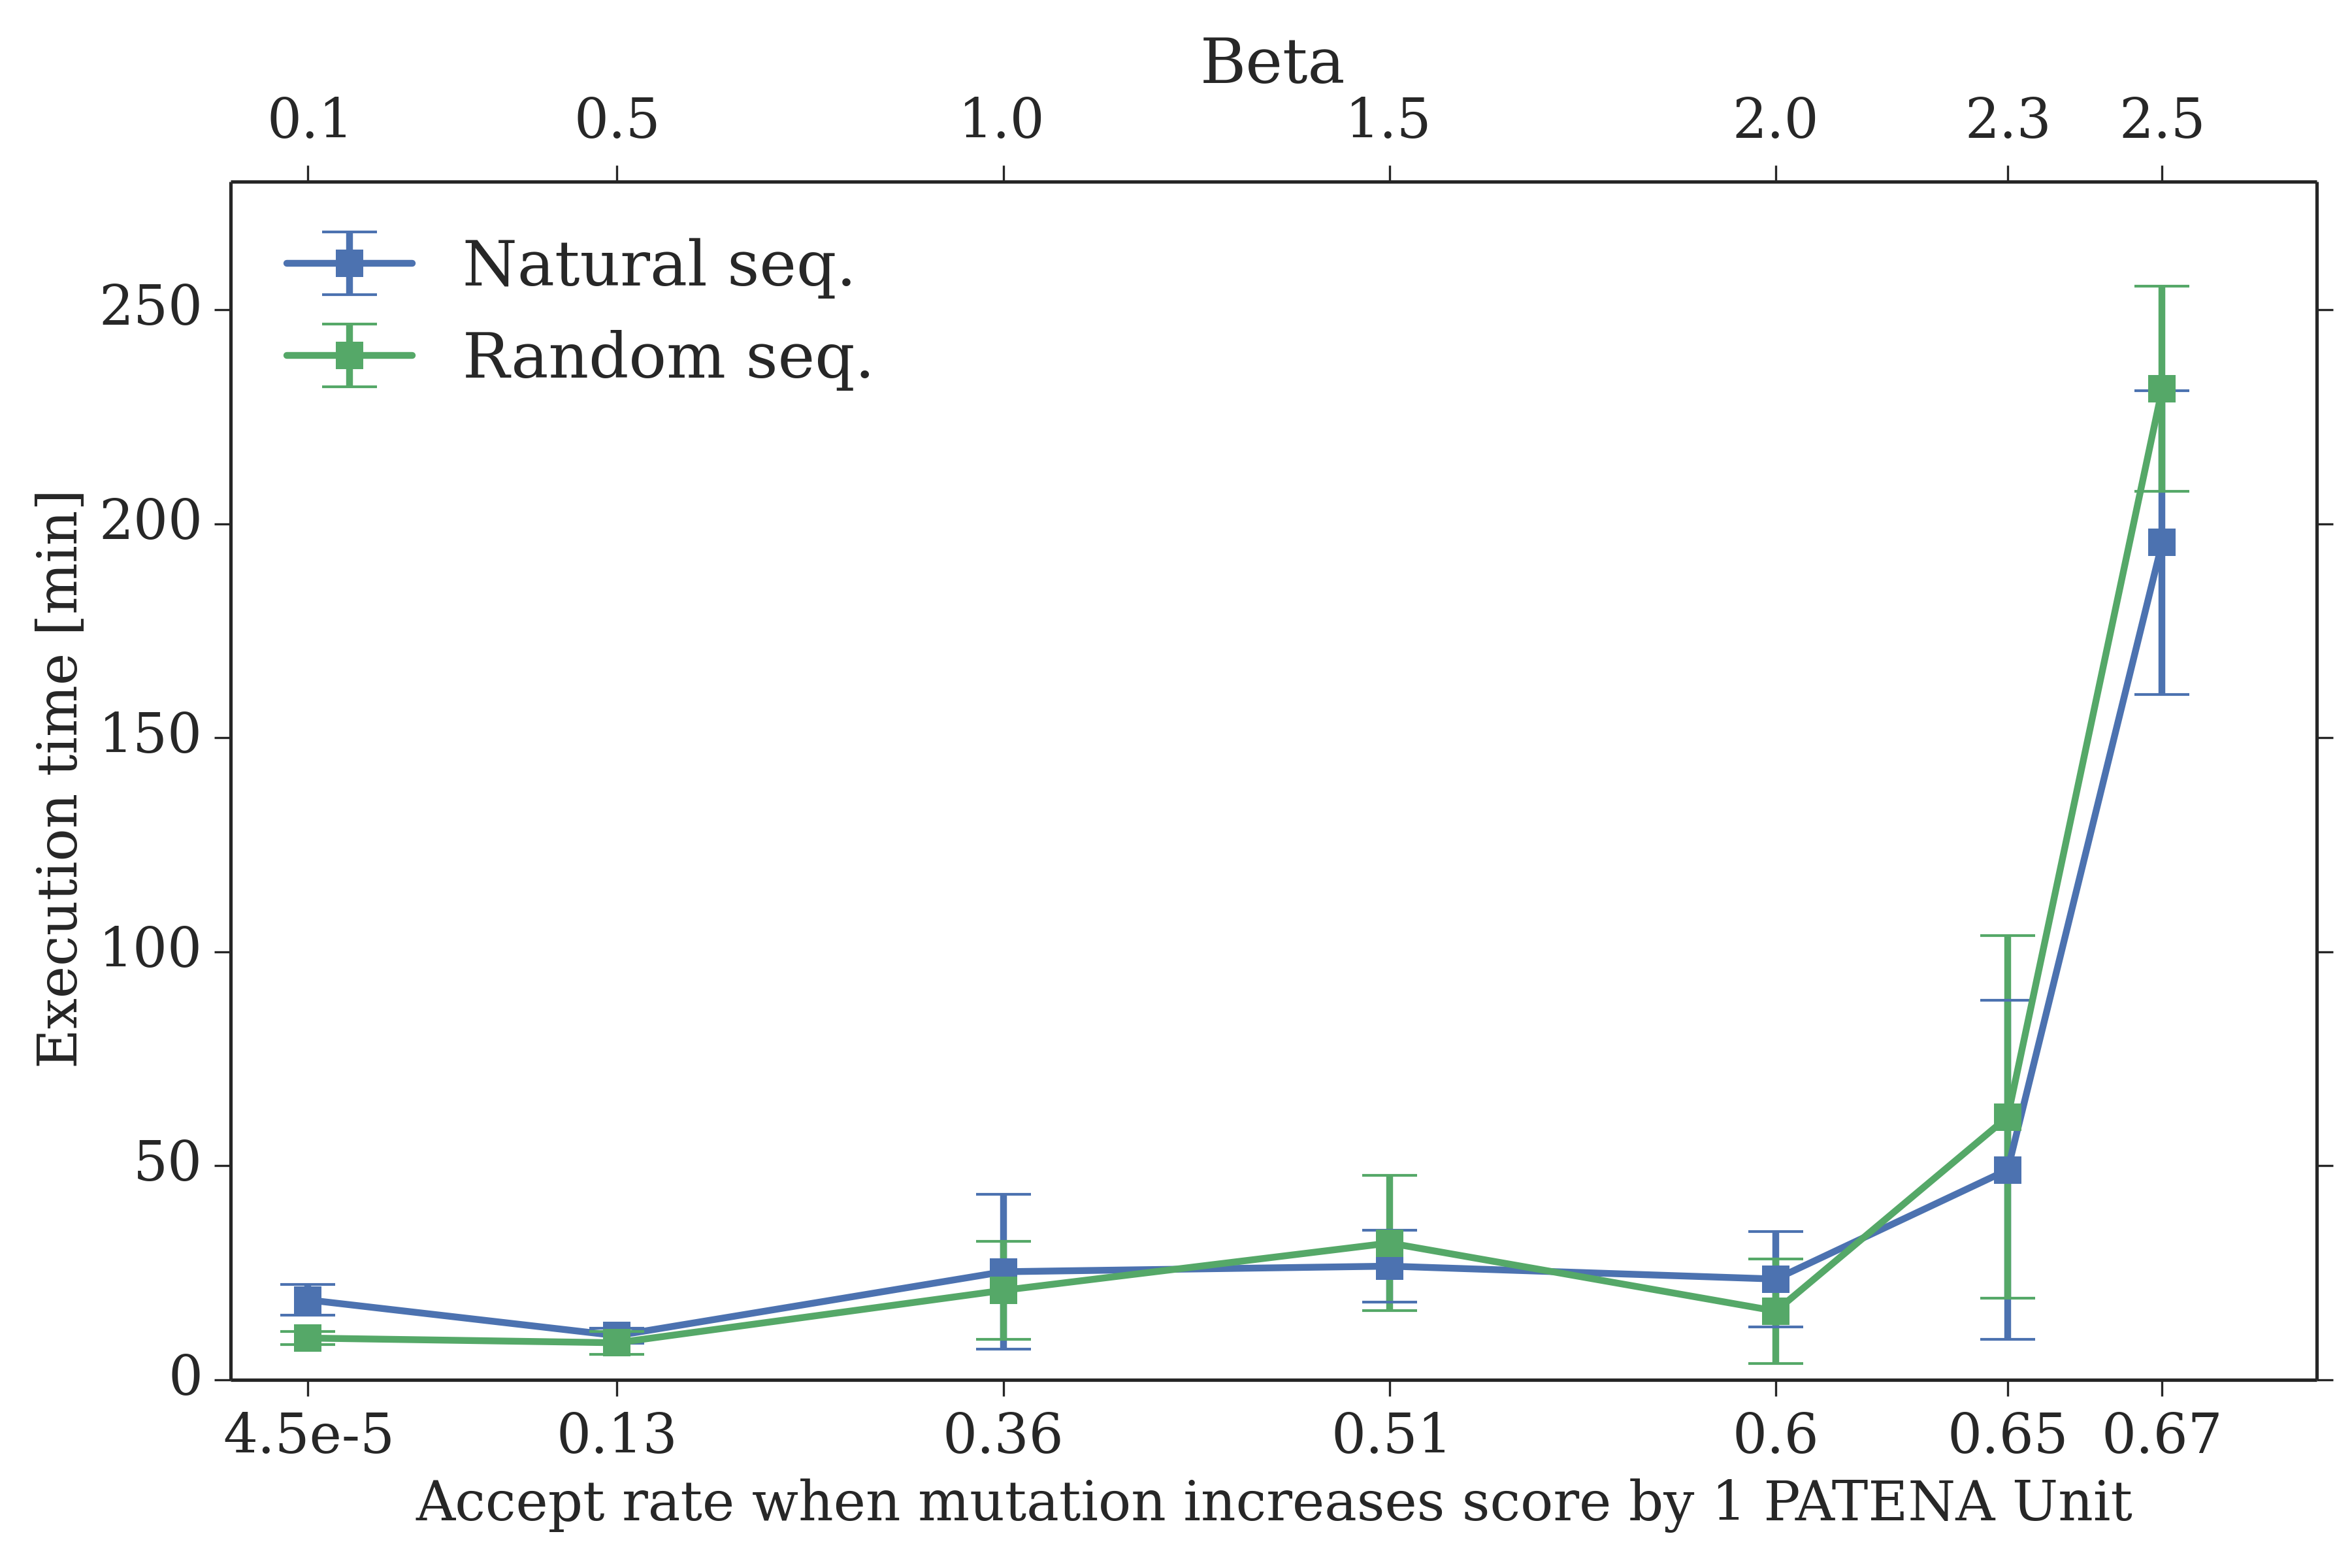
\includegraphics[width=330px,height=210px]{../img/beta-vs-time-length50-300dpi.png} 
\end{adjustwidth}
\end{frame}





% ***************************************************************
%      SCORE vs MUTACION  PARA 1 SOLA EJECUCION USANDO BETA=1.0
% ****************************************************************
\begin{frame}[plain]{Sample execution profile using defined $\beta$ (1.0)}
% \vspace{-0.5\baselineskip}
\begin{adjustwidth}{-1.5em}{-2.5em}
\centering
% \begin{Verbatim}
% How many mutations are required?  - \hspace{5px} Length = 30   
% Length = 30 residues \hspace{5px} - \hspace{5px}   Effect of $\beta$  
% \end{Verbatim}

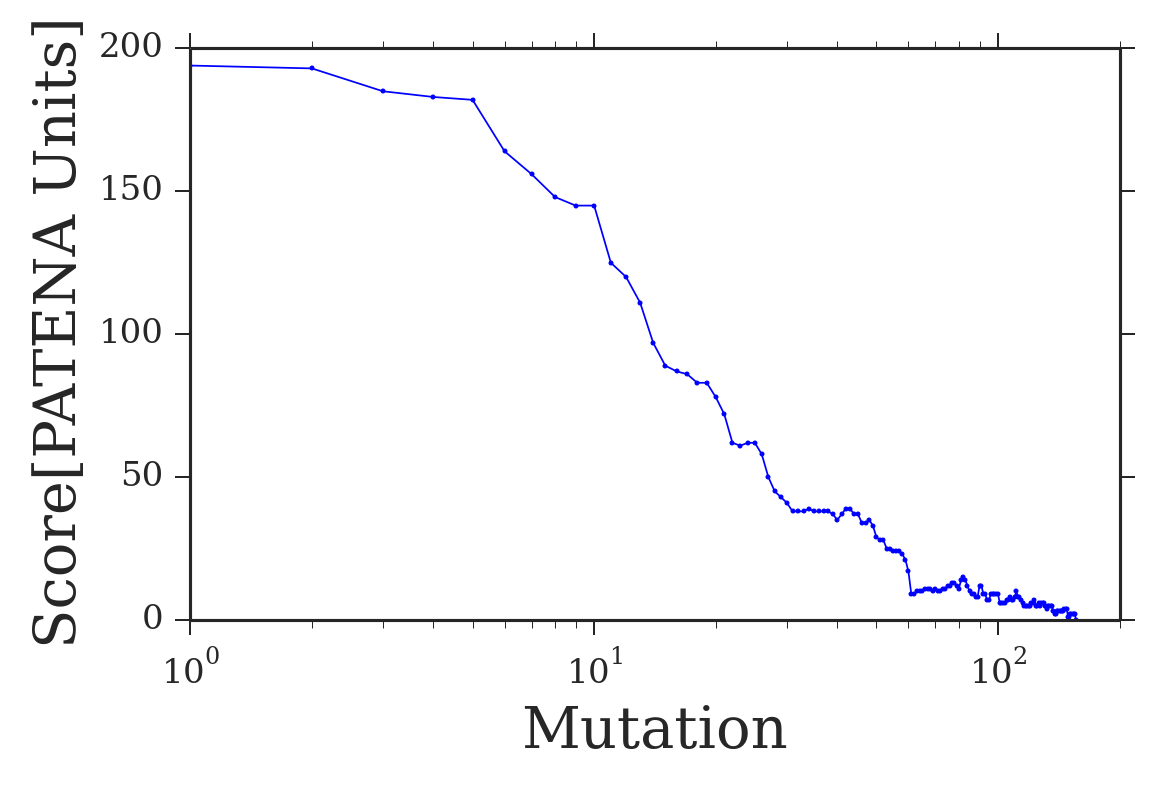
\includegraphics[width=330px,height=210px]{../img/iterationVsScore-individualBeta1-EXAMPLE.png}
% 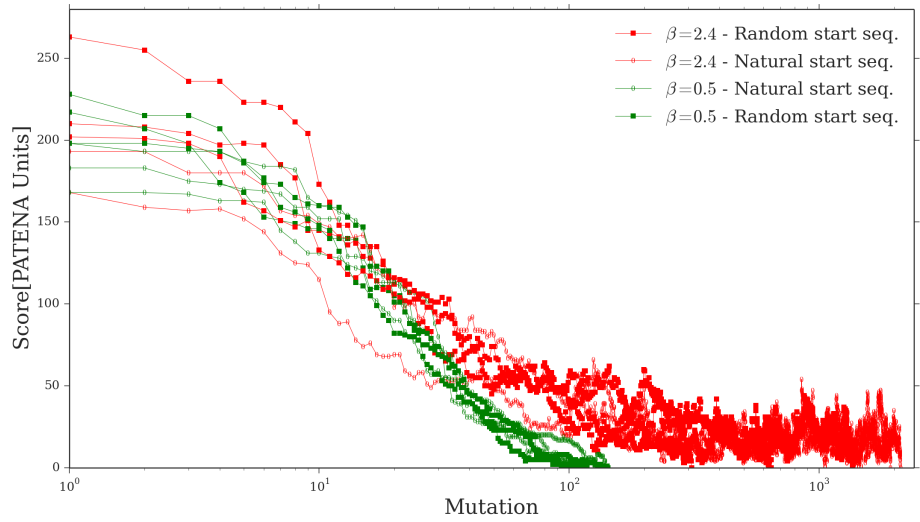
\includegraphics[width=330px,height=210px]{../img/scoreVsMutation-individual.png} 

\end{adjustwidth}
% \vspace{-\baselineskip}
\end{frame}







% *********************************************
%      TIEMPO EJECUCION vs LENGTH SECUENCIA
% *********************************************
\begin{frame}[plain]{Approximate linear dependence with length}
\centering
% Optimal $\beta$ range  
% [Length = 30] - [Random (n=3) and Natural (n=3) seq. / each $\beta$] \\
\begin{adjustwidth}{-1.5em}{-2.5em}
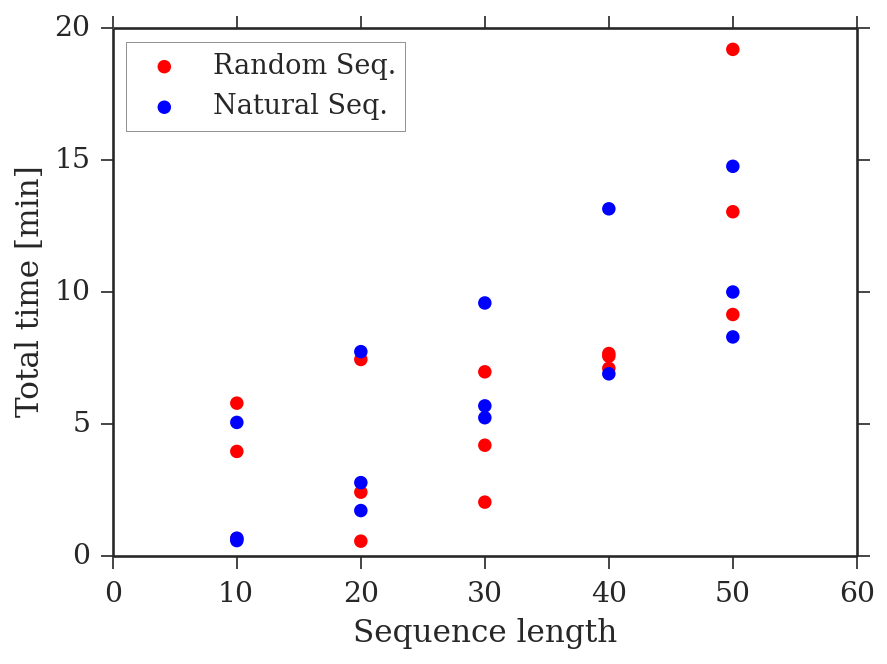
\includegraphics[width=330px,height=210px]{../img/lengthVsTime.png} 
\end{adjustwidth}
\end{frame}





% *********************************************
%      DIVERGENCIA
% *********************************************
\begin{frame}[plain]{Nondeterministic algorithm: same input $\rightarrow$ different results}
\centering
Fixed starting sequence $\rightarrow$ 74 designs\\
\vspace{15px}
\begin{adjustwidth}{-2.5em}{-2.5em}
% \hspace{10px} Identity between resulting designs  \hspace{15px}   Identity against starting seq.
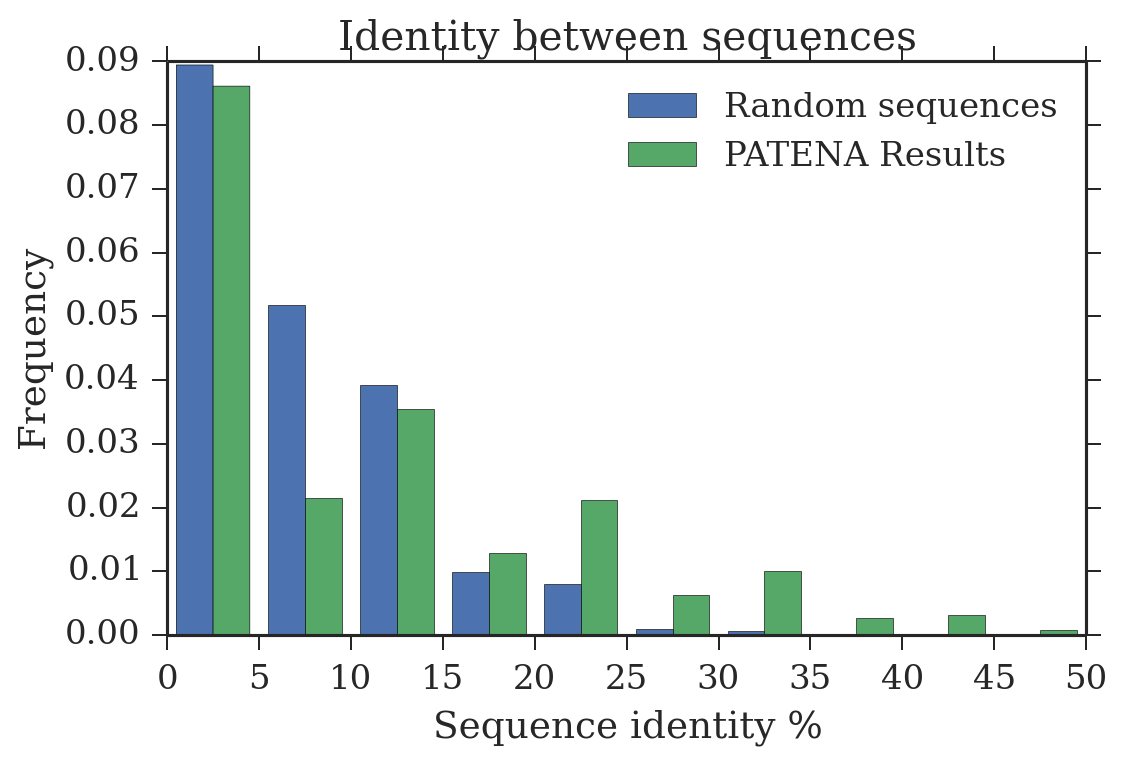
\includegraphics[width=175px,height=145px]{../img/againstAll-random.png}
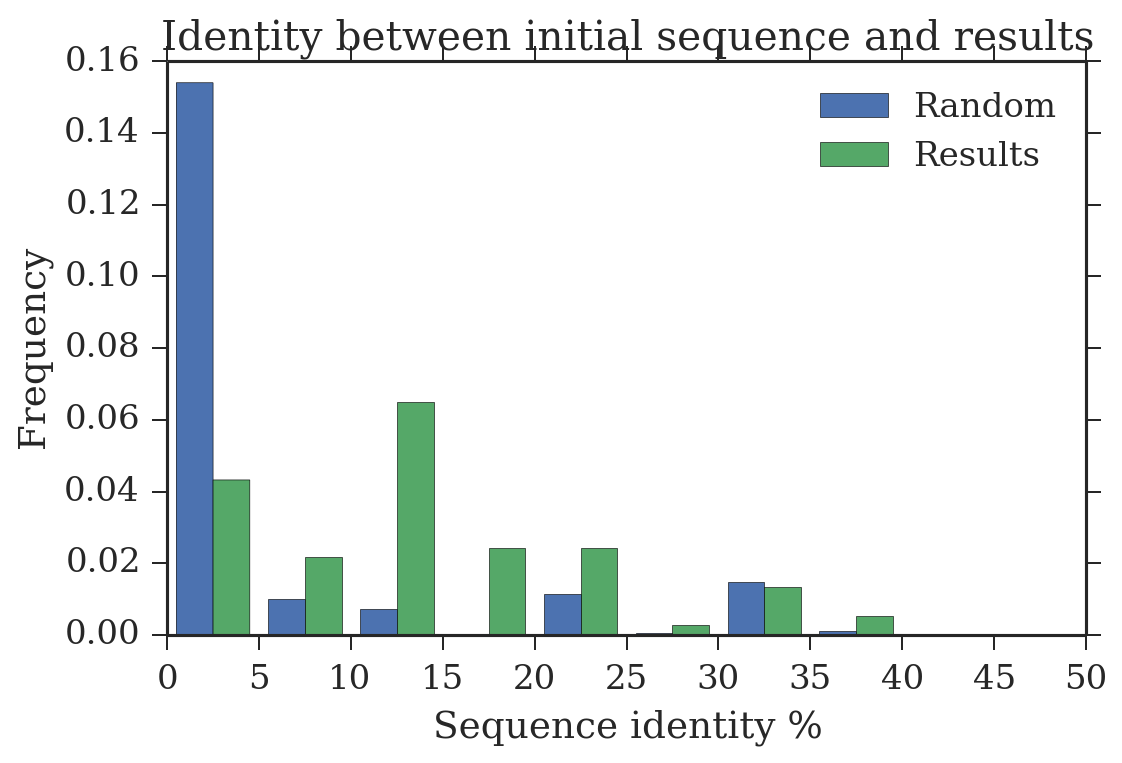
\includegraphics[width=175px,height=145px]{../img/againstInitial-random.png}
\end{adjustwidth}
\end{frame}



\begin{frame}{Conclusion}
\begin{itemize}
 \item PATENA can find suitable protein linkers in a short execution time.
 \item The set of designs that can be obtained from the same sequence shows high diversity. 
 \item Allows for development of server to obtain and collect linker sequences.
%  \item We interpret that the space of suitable linker sequences is a large fraction of the whole sequence space.
\end{itemize}
\end{frame}

















% *************************************************************
% *************************************************************
% *************************************************************
% 			EXTRA
% *************************************************************
% *************************************************************
% *************************************************************







% *************************************************************
% 		 LOGO  
% *************************************************************

\begin{frame}
\centering
Fixed starting sequence $\rightarrow$ 74 designs\\
\begin{adjustwidth}{-1.5em}{-2.5em}
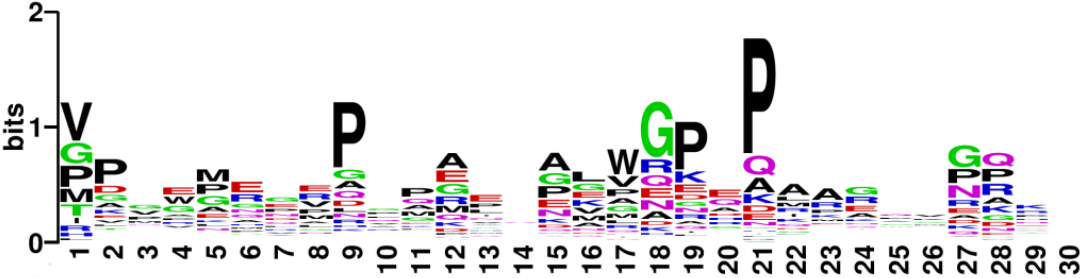
\includegraphics[width=340px,height=150px]{../img/logo.png}\\ 
\vspace{10px}
\hspace{18px}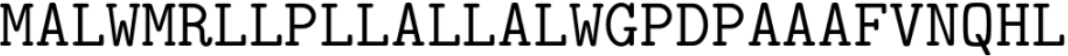
\includegraphics[width=325px,height=15px]{../img/sequence.png}
\end{adjustwidth}
\end{frame}

\begin{frame}
\begin{adjustwidth}{-1.5em}{-2.5em}
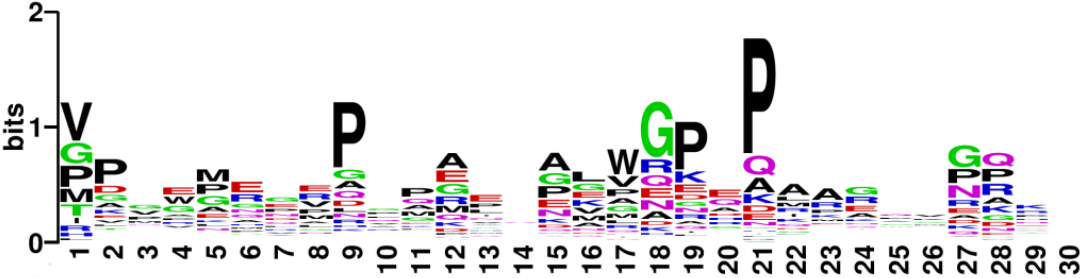
\includegraphics[width=340px,height=150px]{../img/logo.png}\\ 
% \vspace{10px}
\hspace{18px}
\includegraphics[width=325px,height=25px]{../img/sequence2.png}
\end{adjustwidth}
\end{frame}










% *************************************************************
%      OBSERVED FREQUENCY vs EXPECTED FREQUENCY
% *************************************************************
\begin{frame}
% {Standard composition deviation}
\centering
Standard composition
% Fixed starting sequence $\rightarrow$ 74 designs\\
\begin{adjustwidth}{-1.5em}{-2.5em}
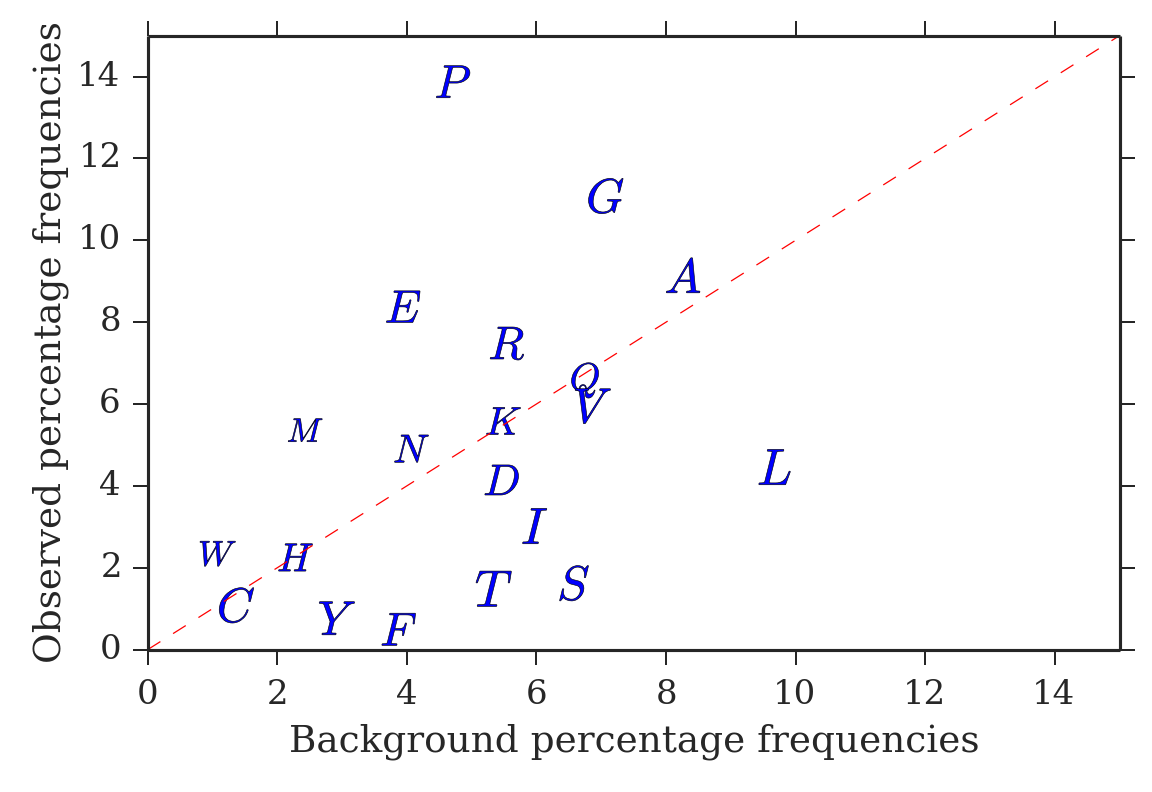
\includegraphics[width=340px,height=250px]{../img/frequenciesComparison.png}\\ 
\end{adjustwidth}
\end{frame}












% *************************************************************
% 		BETA  vs  MUT. ATTEMPTS + ITERATIONS
% *************************************************************
\begin{frame}
\begin{adjustwidth}{-1.5em}{-2.5em}
% 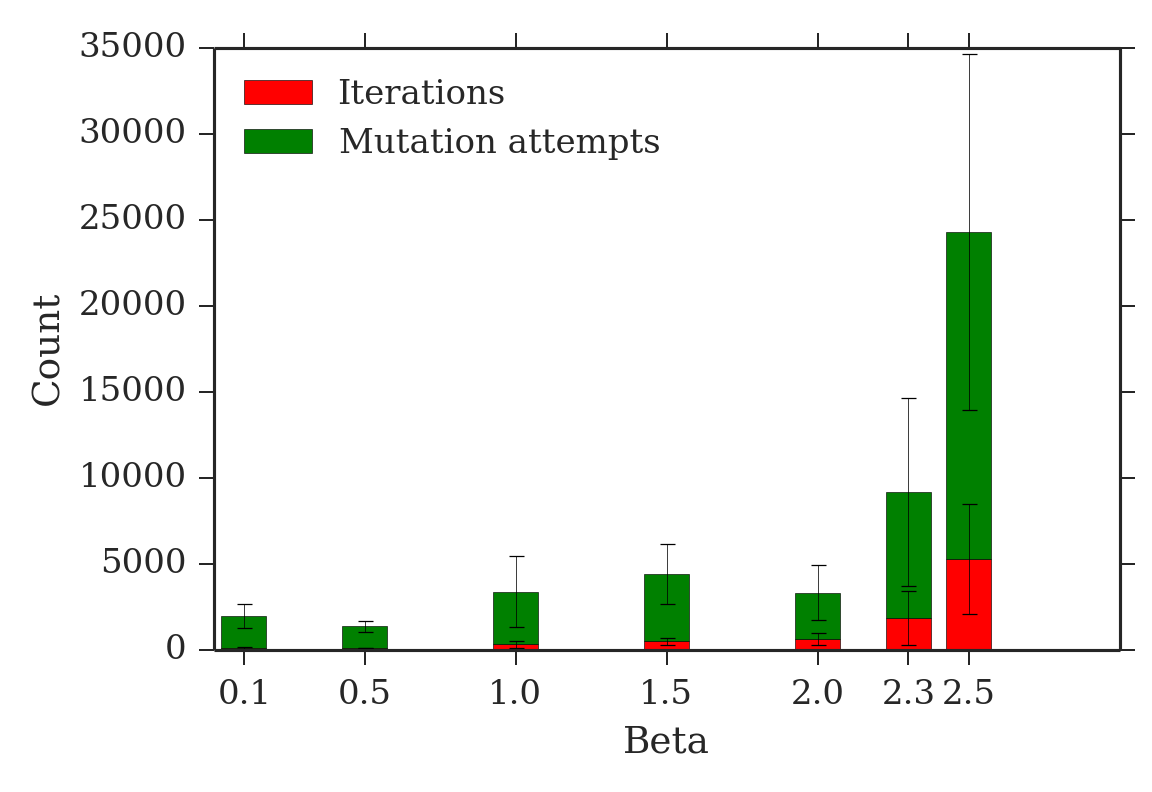
\includegraphics[width=340px,height=250px]{../img/betaVsIterations-MutAttempts.png}\\
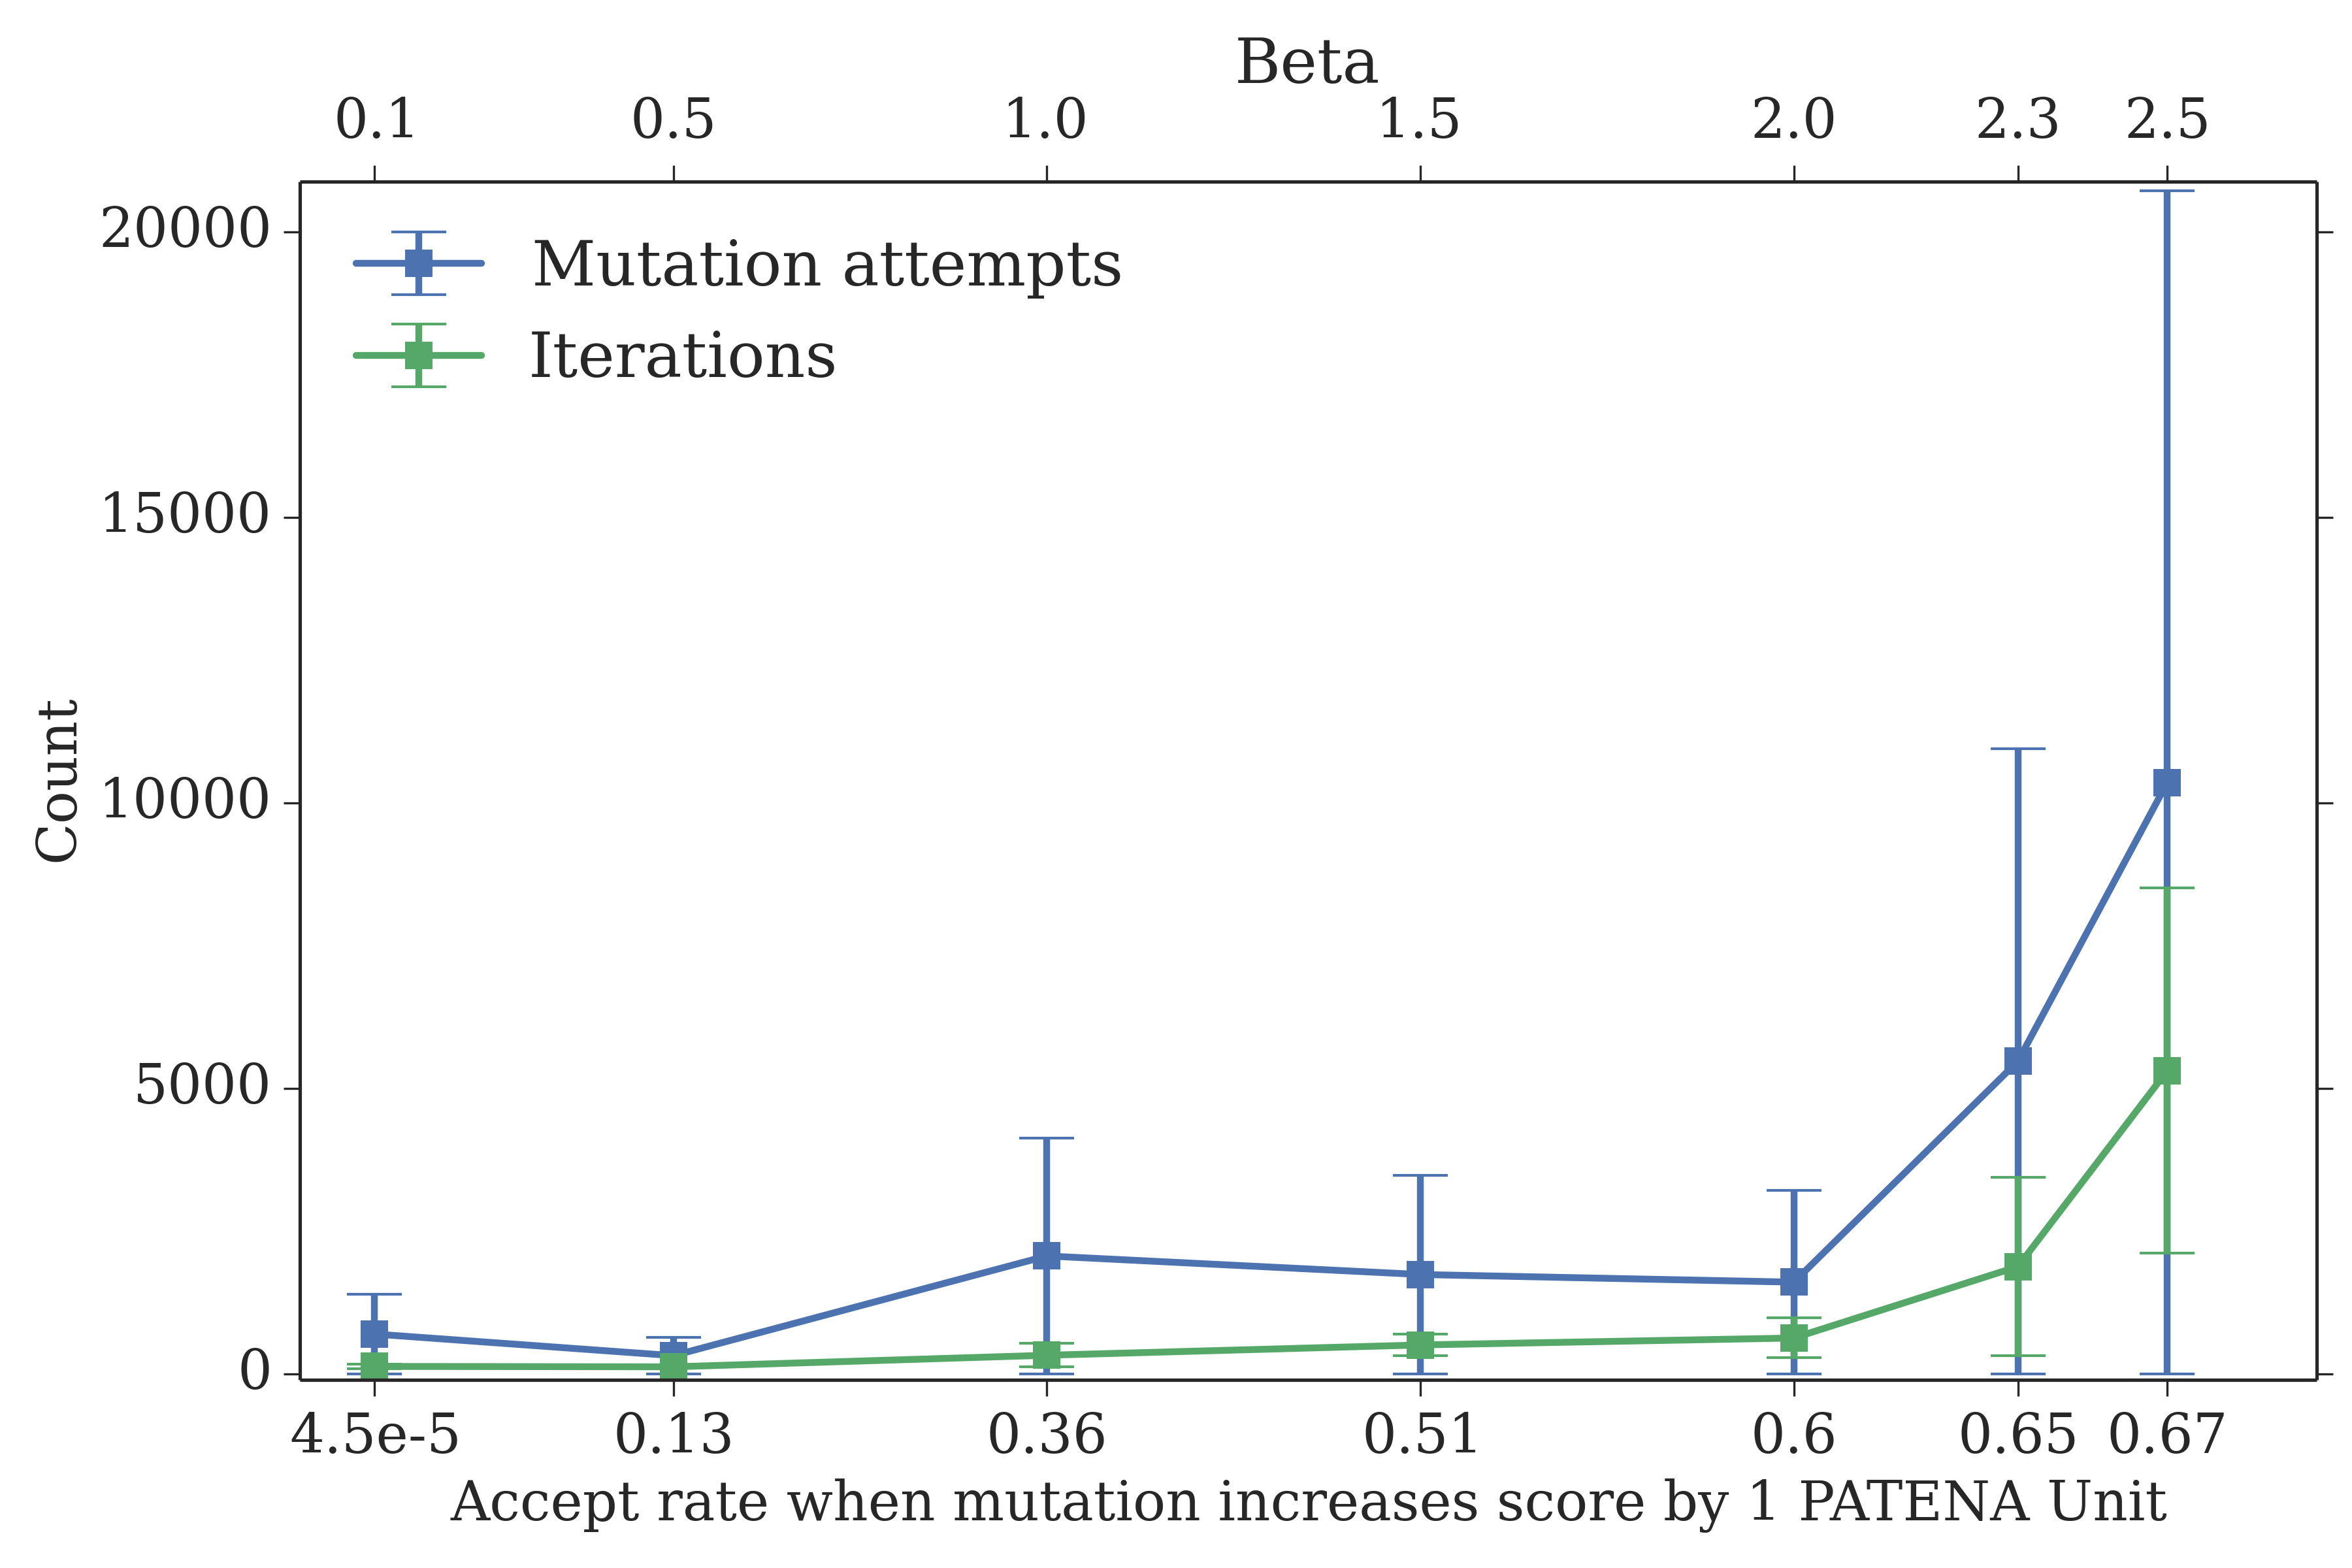
\includegraphics[width=340px,height=250px]{../img/beta-vs-Mut-iterations}\\
\end{adjustwidth}
\end{frame}











% *************************************************************
%     ITERATION vs MUT. ATTEMPTS(MEAN)
% *************************************************************
\begin{frame}
\begin{adjustwidth}{-2.0em}{-2.0em}
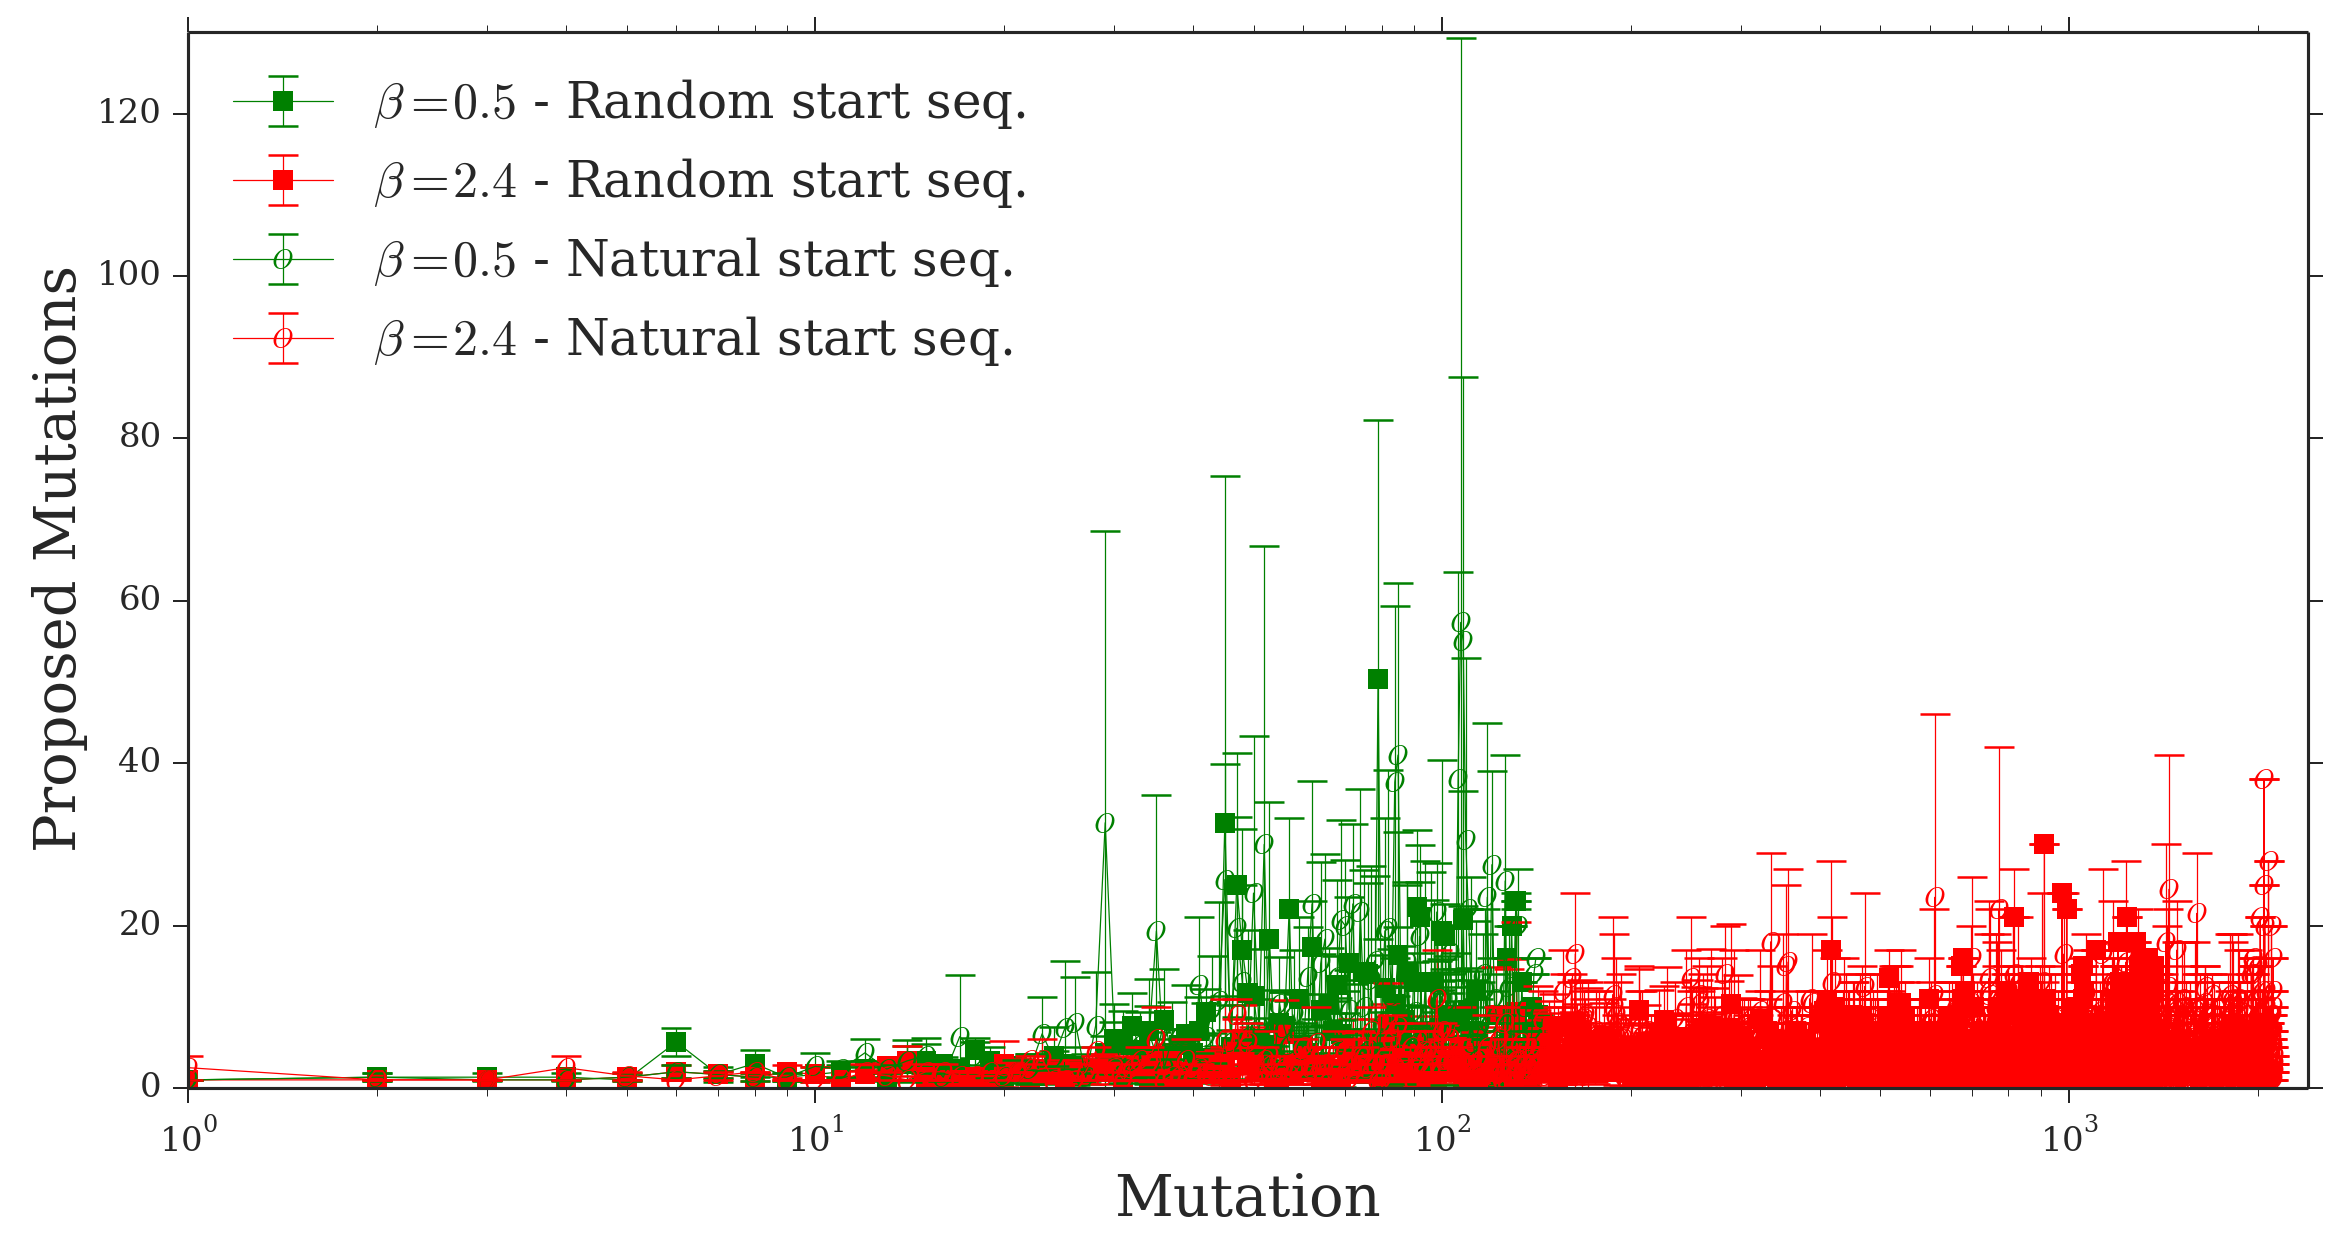
\includegraphics[width=340px,height=250px]{../img/iterationVsMutAttempts-mean.png} 
\end{adjustwidth}
\end{frame}









% 
% \begin{frame}
% \centering
% Fixed starting sequence $\rightarrow$ 74 designs \\
% \begin{adjustwidth}{-1.5em}{-2.5em}
% 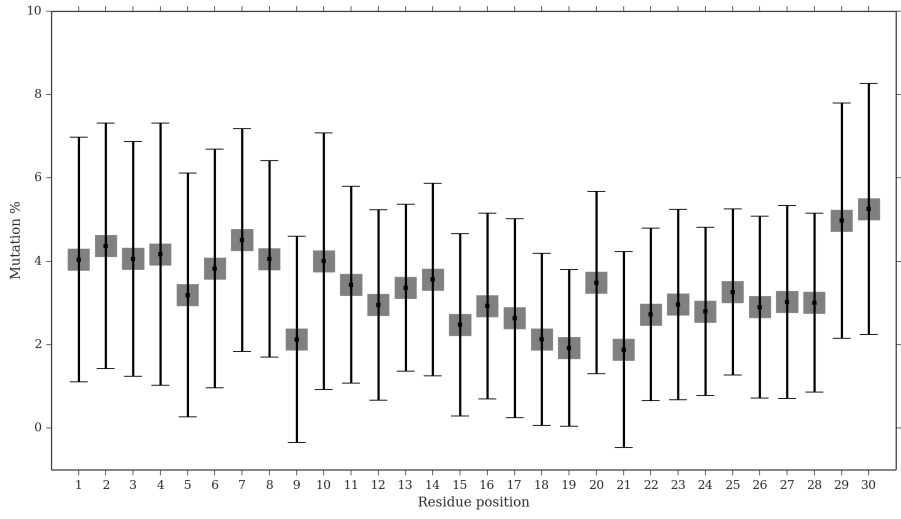
\includegraphics[width=340px,height=150px]{../img/mutationsPerPosition.png}\\ 
% % \vspace{10px}
% \hspace{25px}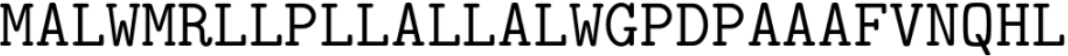
\includegraphics[width=310px,height=10px]{../img/sequence.png}
% \end{adjustwidth}
% \end{frame}
% 





\begin{frame}
\centering
Fixed starting sequence $\rightarrow$ 74 designs - Beta 0.5 , 0.1\\

\begin{adjustwidth}{-1.5em}{-2.5em}
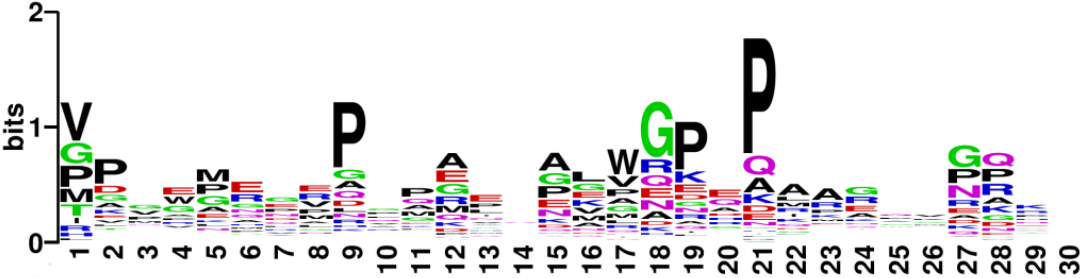
\includegraphics[width=340px,height=80px]{../img/logo.png}\\ 
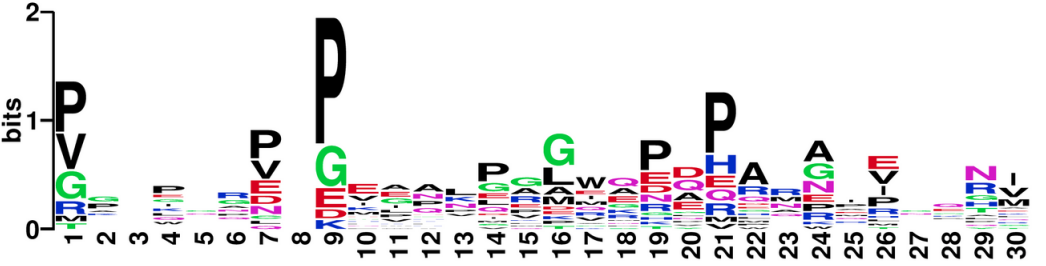
\includegraphics[width=345px,height=80px]{../img/logoBeta0-1.png}\\ 
\vspace{5px}
\hspace{18px}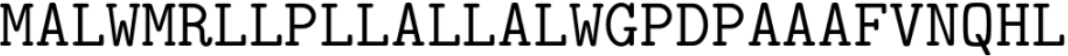
\includegraphics[width=324px,height=15px]{../img/sequence.png}
\end{adjustwidth}
\end{frame}

\end{document}
